\section{Reinforcement learning}

Reinforcement Learning refers to a kind of Machine Learning method in which an agent learns to solve a given task by maximizing the received reward signal, where the agent represents the reinforcement learning algorithm.\\


\begin{figure}[H]
  \centering
  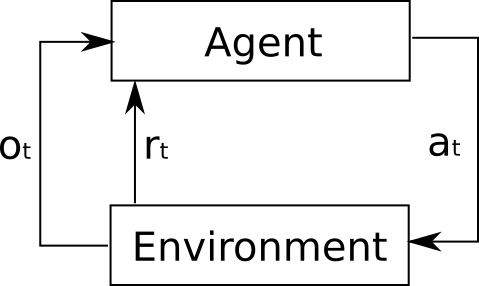
\includegraphics[width=300px]{Images/rl_agent.png} 
  \caption{Agent: reinforcement learning algorithm; Environment: object the agent is acting on; $a_t$: action the agent performes in the environment; $o_t$: observation (current state) of the environment the agent receives; $r_t$: reward signal the agent receives from the environment}
  \label{fig:reinforcement_learning}
\end{figure}


Figure \ref{fig:reinforcement_learning} shows the interaction of the agent with the environment, where the environment refers to the object the agent is acting on. As initial state the agent receives the observation $o_t$ of the environment at time $t = 0$. The observation $o_t$ can be the complete state of the environment, or just a subset of it.
The agent then, based on the observation $o_t$, performs an action $a_t$ in the environment, chosen from a set of possible actions (e.g. moving to the right or moving to the left). After performing the action $a_t$ the agent receives the new observation $o_{t+1}$ of the environment and also the reward signal $r_{t+1}$ which evaluates how good the chosen action was.
Based on the new information the agent again chooses an action $a_t$. The loop continues until the environment sends a termination state.\\

The goal of the agent is to maximize the received reward, which is done by learning an optimal action choosing function called policy, using the received reward signal.
There exist different reinforcement learning algorithms, which all follow the iterative learning algorithm described above, but differ in the update strategy for learning an optimal policy. In the following a short overview over different types of reinforcement learning algorithms will be given.\\

\subsection{Q-learning}

Q-learning is a reinforcement learning algorithm  introduced by Watkins \cite{QLearning} in 1989. 
For any finite markov decision process, Q-learning finds a policy that maximizes the expected total reward over all following steps, starting from the current state.
To do so Q-Learning learns a Q-table, which contains for each state-action pair $(s, a)$ a Q-value representing the expected future reward for taking the action $a$ in state $s$. 
By iteratively updating the Q-value function with the Bellman Equation, the Q-value function will converge to the optimal Q-value function \cite{QLearningProof}.\\

The Bellman Equation 

\begin{equation} \label{eq:bellman_eq1}
Q_{\pi} (s_t, a_t) =\mathbb{E}_{s_{t+1}} [r + \gamma Q_\pi(s_{t+1}, a_{t+1}) | s_t, a_t]
\end{equation}

states, that the Q-value for the state-action pair $(s_t, a_t)$ is equal to the expectation of the received reward $r$, of taking action $a$ in state $s$, plus the discounted future reward the agent will get by following the policy $\pi$ from the next state onwards, where $\gamma$ refers to the discount factor.\\


The optimal Q-value, denoted as $Q^* (s_t, a_t)$ can be expressed as:
\begin{equation} \label{eq:1}
Q^* (s_t, a_t) = \mathbb{E}_{s_{t+1}} [r + \gamma \max_{a_{t+1}} Q^*(s_{t+1}, a_{t+1}) | s_t, a_t]
\end{equation}

After the agent has converged to the optimal policy $Q^* (s_t, a_t)$ it is able to to choose in each possible state the optimal action.\\


\subsection{Value-based versus policy-based reinforcement learning methods}


Value-based methods are learning a value function, which maps state-action pairs directly to values. The best action in a certain state can then be found by taking the action with the biggest value. 
The policy is therefore the action choosing strategy, if the action is always taken by choosing the action with the biggest value the strategy is called greedy.
However if the agent always chooses the greediest action, it will soon get stuck in a local minima and will never be able to find the optimal policy. 
To find the optimal policy the agent needs to explore as many states as possible. 
Thats the reason why usually an $\epsilon$-greedy policy is used, which chooses with a probability of $\epsilon$ a random action, exploration, and otherwise a greedy action, exploitation.
An example of a value-based method is the Q-learning method mentioned in the previous section.\\

Policy-based methods, in contrast to value-based methods, optimize the policy directly without using a value function.
The main problem of policy-based methods is to find a good score function to compute how good a policy is. An example of a policy-based method is reinforcement learning with policy gradient.\\


\subsection{Model-free versus model-based reinforcement learning}

Model-free reinforcement learning maps observations of the environment directly to values or actions.
In contrast to this, model-based reinforcement learning algorithms are using a model of the environment to simulate the dynamics of the environment. The model knows the transition probability $T(s_{t+1} | s_t, a_t)$ to the next state $s_{t+1}$ given the current state $s_t$ and the current action $a_t$. By taking this model into account, adverse consequences of trial-and error can be avoided, also the performance of the agent can be increased by increasing the amount of internal simulations.
But there are some drawbacks. If the model is imperfect the performance of model-based agents suffers. Also it is not always possible to get an exact transition model or to get a transition model at all, especially in real world applications.\\



\subsection{Deep Q network}

In the paper "Human-level control through deep reinforcement learning" Mnih et al. \cite{dqn} introduce the first reinforcement learning algorithm which uses a neuronal network as a function approximator for the Q-value function. Reinforcement learning algorithms, which are using a neuronal network as function approximator, are also called deep reinforcement learning.\\

The approximated target values are

\begin{equation} \label{eq:1}
y = r + \gamma \max_{a_{t+1}} Q(s_{t+1}, a_{t+1}; \theta_i^-)
\end{equation}

The network parameters $\theta_i$ can than be optimized by minimizing the loss between the optimal target values and the approximated target values. Because the optimal target values are not know a second network with fixed weights $\theta_i^-$ is used. The loss function looks as follow:

\begin{equation} \label{eq:dqn_loss}
L_i(\theta_i) = \mathbb{E}_{s, a, r}[(\mathbb{E}_{s_{t+1}} [ y | s, a] - Q(s, a; \theta_i))^2]
\end{equation}


For more details see the paper \cite{dqn}.\\



\subsection{Advantage-actor-critic}
\label{sec:a2c}

Mnih et al. introduce in the paper "Asynchronous Methods for Deep Reinforcement Learning" \cite{A3C} the deep reinforcement learning algorithm asynchronous advantage-actor-critic (A3C). Shortly after introducing A3C, Mnih et al. published a synchronous, deterministic variant of A3C called advantage-actor-critic (A2C) which gives equal performance.
A2C combines value-based and policy-based reinforcement learning and consists of two parts. A critic which measures how good a taken action is (value-based) and an actor which controls how the agent behaves (policy-based).\\

The \textbf{actor} learns the policy function $\pi(a | s, \theta)$, probability of choosing action $a$ given state $s$, which is used to decide the best action $a$ given a specific state $s$.
The actor controls how the agent behaves.
$\theta$ are the learnable weights of the neural network. \\

The \textbf{critic} learns the value function $\mathnormal{V(s, \phi)}$, which measures how good a certain state $s$ is to be in. The value function $V$ is used to calculate the expected cumulative reward $Q(s, a)$ from following the policy $\pi$ from state $s$.
$\phi$ are the learnable weights of the neural network.

\begin{equation}
	Q(s, a) = r_{t+1} + \gamma V^\pi(s_{t+1})
\end{equation}

To update the policy function, the \textbf{Advantage function} is used which tells the improvement of a certain action compared to the average action taken at state $s$. 
In other words, it estimates the improvement of the true reward compared to the expected reward of the current state $s$ by using the temporal difference error:

\begin{equation}
	A(s, a) = Q(s, a) - V(s)
\end{equation}

The advantage function pushes up the probability of an action from a state $s$ if this action was better than the expected value.
This leads to more stability of the learning algorithm and reduces the variance of the estimate, which improves the sample efficience of the algorithm.\\

To learn an optimal policy, we minimize the \textbf{policy $\pi(a | s, \theta)$ loss} function

\begin{equation}
	loss_\pi = - log (\pi_\theta(a | s)) * A
\end{equation}

The \textbf{gradient} of the \textbf{policy $\pi(a | s, \theta)$} loss is therefore

\begin{equation}
	\nabla \theta = A \nabla_\theta log \pi_\theta (a | s)
\end{equation}
	
To learn the value function we minimize the \textbf{value $V(s, w)$ loss}

\begin{equation}
	loss_V = \sum(R - V(s))^2
\end{equation}


